\documentclass{article}

\usepackage{amsmath, amsthm, amssymb, amsfonts}
\usepackage{graphicx}
%It is best practice to keep all your pictures in
%one folder inside the main directory in which your
%TeX file is kept. Here the folder is named "images."
%Replace the name here with your folder's name, if needed.
%The period is needed due to relative referencing.
\graphicspath{ {./images/} }
%If you have JPEG format images, add .jpg as an
%allowed file extension below. Same for Bitmaps (.bmp).
\DeclareGraphicsExtensions{.png}
\usepackage{setspace}
\usepackage{geometry}
\usepackage{float}
\usepackage[hidelinks]{hyperref}
\usepackage[utf8]{inputenc}
\usepackage[english]{babel}
\usepackage{framed}
\usepackage[dvipsnames]{xcolor}
\usepackage{tcolorbox}

\usepackage{color}
\usepackage{bbm}
\usepackage{dsfont}
\usepackage{xspace}


% For natbib-style references, uncomment this.
\usepackage[numbers]{natbib}
% \let\cite=\citet
% Use \citet for textual citations Author [#]
% Use \cite for normal citations
% Use \citep for optional pre/post notes
% Ex: \citep[see][p.~5]{Smith2020} gives (see Smith, [#], p. 5).

\usepackage{array}
\usepackage{enumerate}
\usepackage{enumitem}
\usepackage{ulem}
% \let\cite=\citet
\usepackage{adjustbox}
\usepackage{caption}
\usepackage{subcaption}
\usepackage{siunitx}
\usepackage{algorithm}
\usepackage{algpseudocode}

% Custom definitions
\makeatletter
%EDIT the path to the .sty files as needed
\def\input@path{{../../}} % Adjust relative to the current file
\makeatother
\usepackage{mydef}
\usepackage{xthm}
\usepackage{comments}

% -------------- Project specific commands
\newcommand{\HRule}[1]{\rule{\linewidth}{#1}}
% --------------

% \setstretch{1.2}
\geometry{
    textheight=9in,
    textwidth=5.5in,
    top=1in,
    headheight=12pt,
    headsep=25pt,
    footskip=30pt
}

% ------------------------------------------------------------------------------

\begin{document}

% ------------------------------------------------------------------------------
% Cover Page and ToC
% ------------------------------------------------------------------------------

\title{ \normalsize \textsc{}
		\\ [2.0cm]
		\HRule{1.5pt} \\
		\LARGE \textbf{\uppercase{Elastic Research Journal}
		\HRule{2.0pt} \\ [0.6cm] 
      % \LARGE{Subtitle}
      \vspace*{10\baselineskip}}
		}
\date{}
\author{\textbf{Author} \\ 
		Madison Sheridan}

\maketitle
\newpage

\tableofcontents
\newpage

% ------------------------------------------------------------------------------

\section{10/21/2025}
\subsection{Questions}
\begin{enumerate}
   \item Typo in isotropic case of the stress tensor, Eq. (2.5)? Should this be $\bb - \frac{1}{3}\Tr(\bb)\polI$?
   \item How should the stress function be formulated?  I have seen various formulations
   \begin{itemize}
      \item $\bsigma = 2 \frac{\rho}{\rho_0} F \frac{\partial e}{\partial \bC} F\tr$
      On this implementation in particular, why $\rho_0$ in the denominator?  In \cite[Eq.~17]{kluth-despres-2010} the authors use this formulation without $\rho_0$.
      Does this formulation have a name like the Murnaghan stress tensor?
      \item Murnaghan stress tensor
      \begin{equation}
         \bsigma = 2\rho \frac{\partial e}{\partial \bG} \bG,\quad G = \left(F\tr\right)^{-1} F^{-1}.
      \end{equation}
      This formulation is used in \cite[Sec.~3.2]{favrie_gavrilyuk_saurel_2008}, \cite[Eq.~(14)]{boscheri-loubere-maire-2021}, \cite[p.~176]{gavrilyuk-book}.
   \end{itemize}
   %
   \item Uniaxial tension test case \cite{chaimoon2019}.  I believe that $\bsigma$ needs to be reformulated in terms of the reduced invariants.
   \item Issues with momentum conservation (both cartesian directions for all closure models.)
   \begin{figure}[!htb]
      \centering
      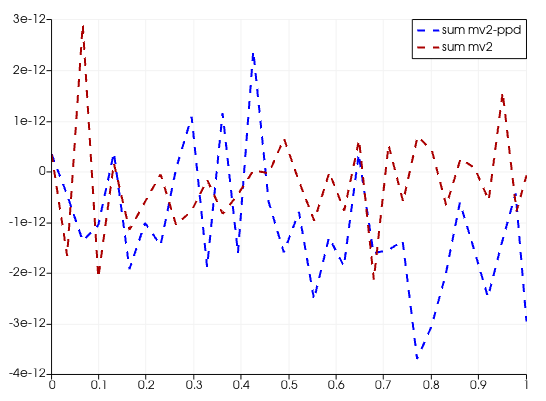
\includegraphics[width=0.6\textwidth]{images/20251021/ivtf1-momentum-y-over-time.png}
      \caption{Exact momentum conservation for IVTF1.}
      % \label{fig:momentum-conservation-error}
   \end{figure}
   \begin{figure}[!htb]
      \centering
      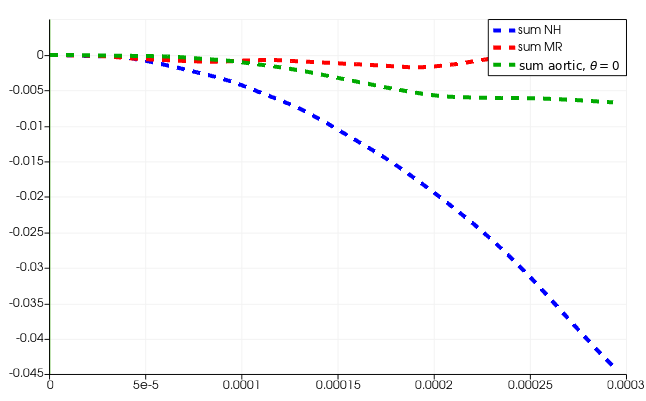
\includegraphics[width=0.6\textwidth]{images/20251021/pp-momentum-y-over-time.png}
      \caption{Momentum conservation error for NH, MR, and uniaxial $\theta=0$.}
      % \label{fig:momentum-conservation-error}
   \end{figure}
   \begin{figure}[!htb]
      \centering
      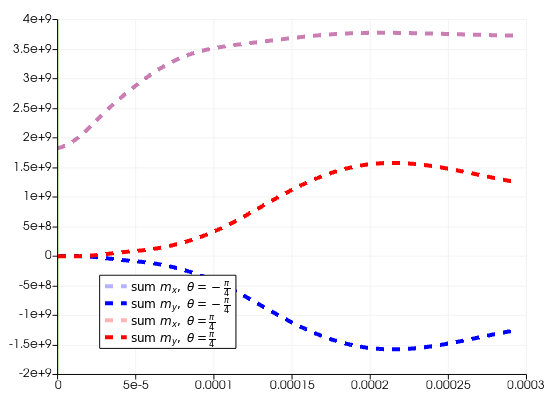
\includegraphics[width=0.6\textwidth]{images/20251021/pp-momentum-xy-over-time-uniaxial.png}
      \caption{Momentum conservation error for uniaxial closure.}
      % \label{fig:momentum-conservation-error}
   \end{figure}
   %
   \item Bonet Burton human leg impact example. Can I run this problem using rectangle shapes in 2D to represent the human leg and wooden beam? Otherwise I am not sure how to handle collapse of air cells between objects initially not in contact.
\end{enumerate}

\subsection{Notes}
First a summary of the discussion addressing the above questions.
\begin{enumerate}
   \item Either is fine. $\Tr\left(\bb\right)$ is the same as $j_1$ so both forms are equivalent.
   \item The Murnaghan stress tensor is fine to be used in the isotropic case since $\bsigma$ is symmetric. The problem is that $bC$ does not commute with $\bG_i$ in the isotropic case, 
   for example for symmetrix matrices $a$ and $G$:
   \begin{align*}
      \left(aG\right)\tr = G\tr a\tr = Ga \neq aG.
   \end{align*} 
   We had a discussion as well on $\partial e / \partial C$ being homogeneous which means it is a polynomial with respect to $\bG_i$ which isn't true.
   \item The Uniaxial test case from \cite{chaimoon2019} is derived in the incompressible case where $\det \bC = 1$ and so $\bc = \bC$.
   Because of this, hyperbolicity is proved in the incompressible case but not guaranteed in the compressible case.
   Hence this is a simplifying assumption for our model, but there is no scaling factor $\det \bC$ that should arise since we adopt the same assumption.
   \item Momentum conservation errors are likely due to the boundary conditions.  
   In particular, the vacuum boundary conditions in the elastic implementation are enforced by setting $\bsigma = \bzero$ on the boundary. 
   Hence the only nonzero entry in the flux at the boundary will be in the update to the specific volume since this is solely dependent on the velocity.
   To check if boundary conditions are the issue, can also run a test case on a large outer square domain with uniform conditions and then prescribe a velocity on a small subset of the domain. 
   Should get exact mass conservation until that small section interacts with the boundary.
   Also consider running the elastic isentropic vortex.
   \item Rectangle mesh is fine. Can also use concrete instead of wood since we have those paramters:
   \begin{align*}
      \gamma &= 4.2 &   p_{\infty} &= 23.9\ (\text{gPa}) \\
      \rho &= 2400\ (\text{kg/m}^3) & \mu &= 13\ (\text{gPa}). \\
   \end{align*}
\end{enumerate}


\newpage

% ------------------------------------------------------------------------------
% Reference and Cited Works
% ------------------------------------------------------------------------------
%fix spacing in bibliography, if any...
%%%%%%%%%%%%%%%%%%%%%%%%%%%%%%%%%%%%%%%%%%%%%%%%%%%%%%%%%%%%%
\let\oldbibitem\bibitem
\renewcommand{\bibitem}{\setlength{\itemsep}{0pt}\oldbibitem}
%%%%%%%%%%%%%%%%%%%%%%%%%%%%%%%%%%%%%%%%%%%%%%%%%%%%%%%%%%%%%%%
%The bibliography style declared is the IEEE format. If
%you require a different style, see the document
%bibstyles.pdf included in this package. This file,
%hosted by the University of Vienna, shows several
%bibliography styles and examples of in-text citation
%and a references page.
% \bibliographystyle{ieeetr}
\bibliographystyle{plainnat}

% \phantomsection
% \addcontentsline{toc}{chapter}{REFERENCES}

% \renewcommand{\bibname}{{\normalsize\rm REFERENCES}}

%This file is a .bib database that contains the sources.
%This removes the dependency on the previous file
%bibliography.tex.
%EDIT the path to the .bib file as needed
\bibliography{../../bibliography}

% ------------------------------------------------------------------------------

\end{document}
